\documentclass[10pt,aspectratio=169]{beamer}
\usetheme{Madrid}
\usecolortheme{dolphin}

\usepackage[utf8]{inputenc}
\usepackage[T1]{fontenc}
\usepackage[spanish,es-noshorthands,es-tabla,es-nodecimaldot]{babel}
\usepackage{booktabs}
\usepackage{array}
\usepackage{tikz}
\usetikzlibrary{arrows.meta,positioning,shapes.geometric,calc}
\usepackage{pgfplots}
\pgfplotsset{compat=1.16}
\usepackage{graphicx}

\setbeamertemplate{navigation symbols}{}
\setbeamertemplate{itemize items}[circle]
\setbeamerfont{caption}{size=\scriptsize}

% Recuadro de síntesis al pie de la lámina: \sintesis{título}{texto}
\newcommand{\sintesis}[2]{%
  \begin{block}{#1}#2\end{block}}

\title[Efecto del diplomado: encuadre y datos]{Efecto del Diplomado en Docencia para la Educación Superior\\ sobre los resultados de los cursos}
\subtitle{Encuadre del problema y análisis inicial de datos}
\author[G. Repetto y J. Pérez]{Gabriela Repetto \and Josefina Pérez}
\institute[ICS3564]{ICS3564 Econometría Avanzada\\ Pontificia Universidad Católica de Chile}
\date[19 nov 2026]{Reunión de validación · 19 de noviembre de 2026}

\begin{document}

% ============================================================
\begin{frame}
  \titlepage
\end{frame}

% ============================================================
\begin{frame}{Objetivo de esta reunión}
  Venimos a validar con ustedes, \alert{antes de construir los modelos finales}, tres cosas:
  \vspace{0.6em}
  \begin{enumerate}
    \item \textbf{El encuadre:} que el problema que estamos abordando sea el que les importa a ustedes, y que la solución que proponemos responda a él.
    \item \textbf{La factibilidad:} qué permiten medir los datos que nos entregaron, y con qué límites.
    \item \textbf{Las decisiones pendientes:} hay definiciones que dependen de cómo funciona la institución, no de la econometría. Para esas necesitamos su criterio.
  \end{enumerate}
  \vspace{0.6em}
  \sintesis{Qué traemos y qué no}{Hoy no traemos una respuesta sobre si el diplomado funciona. Traemos una propuesta de cómo responderlo y una revisión honesta de lo que los datos permiten.}
\end{frame}

\begin{frame}{Contenido}
  \tableofcontents
\end{frame}

% ============================================================
\section{Encuadre: problema y solución}
% ============================================================

\begin{frame}{Contexto: la trayectoria formativa docente}
  \begin{center}
  \begin{tikzpicture}[
      nivel/.style={rectangle, rounded corners, draw=blue!50!black, fill=blue!8, minimum width=3.6cm, minimum height=1.3cm, align=center, font=\small},
      flecha/.style={-{Stealth[length=3mm]}, thick, blue!50!black}]
    \node[nivel] (ini) {\textbf{Inicial}\\ 3 cursos};
    \node[nivel, right=1.1cm of ini] (hab) {\textbf{Habilitante}\\ 10 talleres de metodologías\\ activas + 3 cursos};
    \node[nivel, right=1.1cm of hab, fill=orange!20, draw=orange!60!black] (pro) {\textbf{Profesionalizante}\\ Diplomado};
    \draw[flecha] (ini) -- (hab);
    \draw[flecha] (hab) -- (pro);
  \end{tikzpicture}
  \end{center}
  \vspace{0.3em}
  \begin{columns}[T]
    \begin{column}{0.5\textwidth}
      \textbf{El diplomado}
      \begin{itemize}\small
        \item Cuatro módulos: modelo educativo, talleres de metodologías activas, planificación y evaluación, e innovación docente.
        \item 196 horas en su diseño original y 176 en las dos últimas versiones.
        \item Gratuito, semipresencial, con carta de compromiso de la jefatura.
      \end{itemize}
    \end{column}
    \begin{column}{0.5\textwidth}
      \textbf{Lo que muestran los registros}
      \begin{itemize}\small
        \item Cinco versiones terminadas y la sexta empieza en noviembre de 2026.
        \item Cada versión parte con unos 20 docentes y termina cerca de la mitad.
        \item \alert{47 docentes aprobados} con certificado entre 2023 y 2026.
      \end{itemize}
    \end{column}
  \end{columns}
\end{frame}

\begin{frame}{El problema que entendemos que tienen ustedes}
  \begin{block}{La necesidad, según lo planteado en la reunión del 17 de noviembre}
    Saber \textbf{cómo impactan las formaciones docentes en la experiencia de aprendizaje de los estudiantes}, con una solución que sea \textbf{replicable} para la nueva trayectoria formativa que se espera para 2027.
  \end{block}
  \vspace{0.4em}
  \textbf{Por qué hoy no se puede responder}
  \begin{itemize}
    \item La institución ofrece unas 17 instancias formativas y no tiene una forma común de medir su efecto sobre los estudiantes.
    \item Existe un modelo de evaluación anterior, creado por un consultor, que estaba pensado solo para el diplomado y no estaba suficientemente contextualizado.
    \item Los datos existen (notas, carga docente y formaciones aprobadas), pero están en tres bases separadas que hay que unir para responder la pregunta.
  \end{itemize}
  \vspace{0.3em}
  \sintesis{La brecha que queremos cerrar}{La oferta formativa es amplia, pero no hay una forma común de medir si cambia algo en los cursos de los docentes que participan. Esa es la brecha que queremos empezar a cerrar.}
\end{frame}

\begin{frame}{Nuestra pregunta y qué medimos}
  \begin{block}{Pregunta}
    ¿Cambian los resultados de los cursos que dicta un docente \textbf{después} de que aprueba el diplomado?
  \end{block}
  \begin{columns}[T]
    \begin{column}{0.5\textwidth}
      \textbf{Resultados que usamos}
      \begin{itemize}\small
        \item \textbf{Promedio del curso:} nota final promedio de los estudiantes de cada sección.
        \item \textbf{Tasa de aprobación:} proporción de estudiantes que aprueban la sección.
      \end{itemize}
    \end{column}
    \begin{column}{0.5\textwidth}
      \textbf{Lo que este estudio no responde}
      \begin{itemize}\small
        \item Si cambió el aprendizaje profundo o la experiencia del estudiante en sentido amplio.
        \item Si cambió la práctica del docente en la sala.
        \item Por eso coincide con la idea de un \textbf{enfoque mixto}: esto sería la pieza cuantitativa.
      \end{itemize}
    \end{column}
  \end{columns}
  \vspace{0.3em}
  \begin{alertblock}{Una advertencia importante}
    La nota la pone el mismo docente, y el módulo 3 del diplomado trabaja justamente el diseño de la evaluación. Si las notas cambian, puede ser porque cambió el aprendizaje \emph{o} porque cambió la forma de evaluar. Con estos datos no podemos separar ambas cosas.
  \end{alertblock}
\end{frame}

\begin{frame}{Cómo se ha abordado antes}
  \textbf{En la institución}
  \begin{itemize}
    \item Un modelo de evaluación de un consultor, específico del diplomado y basado en instancias del propio programa.
  \end{itemize}
  \vspace{0.4em}
  \textbf{En la investigación}
  \begin{itemize}
    \item \textbf{Angrist y Lavy (2001)} evaluaron una capacitación docente en escuelas de Jerusalén. Compararon la evolución de los resultados de los estudiantes en escuelas que recibieron la capacitación con escuelas parecidas que no la recibieron, antes y después.
    \item Nuestro caso agrega una dificultad: los docentes \textbf{entran en distintos años} (versiones 2023, 2024, 2025 y 2026). Para eso hay métodos recientes de \textbf{diferencias en diferencias escalonadas} (Callaway y Sant'Anna, 2021; Sun y Abraham, 2021), que corrigen problemas conocidos del método tradicional (Goodman-Bacon, 2021).
  \end{itemize}
  \vspace{0.3em}
  \sintesis{Qué tomamos de ese trabajo}{Replicamos la lógica de Angrist y Lavy, comparar cambios y no niveles, con herramientas pensadas para participantes que entran en momentos distintos.}
\end{frame}

\begin{frame}{La solución conceptual: comparar cambios, no niveles}
  \begin{columns}[c]
    \begin{column}{0.52\textwidth}
      \begin{tikzpicture}
        \begin{axis}[width=7.2cm, height=5.0cm, xmin=0.5, xmax=4.9, ymin=4.4, ymax=5.9,
            xtick={1,2,3,4}, xticklabels={Año 1,Año 2,Año 3,Año 4}, ytick=\empty,
            ylabel={Resultado del curso}, axis lines=left, legend columns=1,
            legend style={at={(0.5,-0.2)},anchor=north,font=\scriptsize,draw=none}]
          \addplot[thick, orange!80!black, mark=*] coordinates {(1,5.0) (2,5.1) (3,5.5) (4,5.6)};
          \addlegendentry{Docentes del diplomado}
          \addplot[thick, blue!60!black, mark=square*] coordinates {(1,4.7) (2,4.8) (3,4.9) (4,5.0)};
          \addlegendentry{Docentes que aún no lo hacen}
          \addplot[thick, dashed, orange!60!black] coordinates {(2,5.1) (3,5.2) (4,5.3)};
          \addlegendentry{Sin diplomado (contrafactual)}
          \draw[dotted, thick] (axis cs:2.5,4.4) -- (axis cs:2.5,5.9);
          \node[font=\scriptsize, align=center] at (axis cs:2.5,4.52) {diplomado};
          \draw[{Stealth}-{Stealth}, red!70!black, thick] (axis cs:4.15,5.3) -- (axis cs:4.15,5.6);
          \node[font=\scriptsize, red!70!black, anchor=west] at (axis cs:4.18,5.45) {efecto};
        \end{axis}
      \end{tikzpicture}\par
      {\scriptsize Gráfico ilustrativo, no son datos reales.}
    \end{column}
    \begin{column}{0.46\textwidth}
      \small
      \textbf{Por qué no basta comparar participantes con no participantes}
      \begin{itemize}
        \item Quienes llegan al diplomado no son al azar: postulan con carta de su jefatura y muchos son invitados directamente.
        \item Pueden ser docentes distintos desde antes (más motivados, otras carreras).
      \end{itemize}
      \textbf{Qué hacemos}
      \begin{itemize}
        \item Seguimos a cada docente en el tiempo y miramos \textbf{cuánto cambian} sus cursos después del diplomado.
        \item Ese cambio lo comparamos con el de docentes que todavía no han hecho el diplomado en ese momento.
      \end{itemize}
    \end{column}
  \end{columns}
\end{frame}

\begin{frame}{Valor aplicado y potencial de transferencia}
  \textbf{Lo que entregamos no es solo un número, es un procedimiento}
  \begin{itemize}
    \item Código que une las tres bases, aplica reglas explícitas y documentadas, y estima el efecto.
    \item Se puede volver a correr cada vez que llegan datos nuevos (por ejemplo, la versión 6).
    \item Se puede aplicar a \textbf{otra formación} de la trayectoria cambiando un solo parámetro: sirve para la nueva trayectoria de 2027.
  \end{itemize}
  \vspace{0.4em}
  \textbf{Dos pruebas que nos pidieron}
  \begin{itemize}
    \item \textbf{Trade-off:} mismo diplomado, varias formas de modelar. Vemos si la conclusión depende de nuestras decisiones.
    \item \textbf{Sensibilidad:} mismo procedimiento aplicado a otra formación. Vemos si el método funciona fuera del diplomado.
  \end{itemize}
  \vspace{0.3em}
  \sintesis{Qué le queda a la unidad}{El valor está en tener una forma replicable y transparente de mirar el efecto de cualquier formación, no solo en el resultado de esta evaluación.}
\end{frame}

% ============================================================
\section{Análisis inicial de datos}
% ============================================================

\begin{frame}{Las tres bases y cómo se conectan}
  \begin{center}
  \begin{tikzpicture}[
      base/.style={rectangle, rounded corners, draw=blue!50!black, fill=blue!8, minimum width=3.1cm, minimum height=1.6cm, align=center, font=\small},
      llave/.style={font=\tiny, align=center}]
    \node[base] (perf) {\textbf{Perfeccionamiento}\\ quién aprobó qué formación\\ y en qué año};
    \node[base, right=2.5cm of perf, fill=orange!15, draw=orange!60!black] (carga) {\textbf{Carga docente}\\ qué docente dictó\\ cada sección};
    \node[base, right=2.5cm of carga] (rend) {\textbf{Rendimiento}\\ nota de cada estudiante\\ en cada sección};
    \draw[very thick, blue!50!black] (perf) -- node[llave, above=2pt] {docente\\(RUT anonimizado + DV)} (carga);
    \draw[very thick, blue!50!black] (carga) -- node[llave, above=2pt] {sección\\(período + NRC)} (rend);
  \end{tikzpicture}
  \end{center}
  \vspace{0.6em}
  \begin{columns}[T]
    \begin{column}{0.33\textwidth}\small\centering
      2.353 formaciones aprobadas\\ 47 del diplomado
    \end{column}
    \begin{column}{0.33\textwidth}\small\centering
      55.485 filas · 27.106 secciones\\ 3.314 docentes · 2021--2026
    \end{column}
    \begin{column}{0.33\textwidth}\small\centering
      467.100 notas · 2021 a 202615\\ (2026 todavía incompleto)
    \end{column}
  \end{columns}
  \vspace{0.6em}
  \sintesis{Por qué la carga docente es central}{La carga docente es el puente: dice qué docente dictó cada sección y así podemos conectar las formaciones del docente con las notas de sus estudiantes.}
\end{frame}

\begin{frame}{Limpieza de la base de notas}
  \begin{columns}[c]
    \begin{column}{0.55\textwidth}
      \begin{table}\small
        \begin{tabular}{lr}
          \toprule
          Paso & Filas \\
          \midrule
          Notas en las seis hojas & 467.100 \\
          -- Copia de 202520 y 202525 en la hoja 2026 & 33.974 \\
          -- Sección sin código válido (vacía o tipo SG) & 9.363 \\
          -- Notas pendientes & 356 \\
          -- Programas de postgrado & 8 \\
          \midrule
          \textbf{Matrículas para el análisis} & \textbf{423.399} \\
          \bottomrule
        \end{tabular}
      \end{table}
    \end{column}
    \begin{column}{0.43\textwidth}\small
      \begin{itemize}
        \item Los períodos 202520 y 202525 venían repetidos en las hojas 2025 y 2026. Por indicación de Ricardo, usamos la copia de la hoja 2025.
        \item \alert{El 97,8 \%} de las matrículas encuentra su sección en la carga docente.
        \item En la carga dejamos solo componentes activos y con nota (acuerdo sobre laboratorios), y excluimos los períodos 30, 35 y 90, que no tienen notas.
      \end{itemize}
    \end{column}
  \end{columns}
  \vspace{0.4em}
  \sintesis{Estado de las bases}{Las bases están en buen estado: casi todas las notas se pueden asignar a un docente.}
\end{frame}

\begin{frame}{Los docentes del diplomado en los datos}
  \begin{columns}[c]
    \begin{column}{0.5\textwidth}
      \begin{table}\small
        \begin{tabular}{lccc}
          \toprule
          Año del & Aprobados & En la carga & Con cursos antes \\
          certificado & & docente & y después \\
          \midrule
          2023 & 15 & 15 & 12 \\
          2024 & 19 & 19 & 15 \\
          2025 & 7 & 7 & 5 \\
          2026 & 6 & 6 & 0 \\
          \midrule
          Total & 47 & 47 & 32 \\
          \bottomrule
        \end{tabular}
      \end{table}
      {\scriptsize ``Antes y después'': al menos una sección con 5 o más estudiantes en un año anterior y en uno posterior al certificado. Cinco docentes tenían un error de tipeo en el RUT, ya corregido con Ricardo.}
    \end{column}
    \begin{column}{0.48\textwidth}
      \begin{center}
      \begin{tikzpicture}[caja/.style={rectangle, draw=blue!50!black, fill=blue!8, align=center, font=\small, minimum height=0.8cm}]
        \node[caja, minimum width=5.2cm] (a) {47 aprobaron el diplomado};
        \node[caja, minimum width=4.4cm, below=0.25cm of a] (b) {47 dictan cursos en la institución};
        \node[caja, minimum width=3.6cm, below=0.25cm of b] (c) {32 se pueden comparar\\ antes y después};
        \node[caja, minimum width=2.8cm, below=0.25cm of c, fill=orange!20, draw=orange!60!black] (d) {20 si solo usamos\\ secciones de un docente};
      \end{tikzpicture}
      \end{center}
    \end{column}
  \end{columns}
  \vspace{0.3em}
  \sintesis{Cuántos docentes sostienen la evaluación}{La evaluación descansa en entre 20 y 32 docentes. Es un número chico, y eso limita qué tan finos pueden ser los resultados.}
\end{frame}

\begin{frame}{Desafío 1: secciones con más de un docente}
  \begin{columns}[T]
    \begin{column}{0.48\textwidth}\small
      \textbf{Qué encontramos}
      \begin{itemize}
        \item Casi la mitad de los pares sección--docente está en secciones con más de un docente.
        \item En el 70 \% de esos casos, todos los docentes aparecen en el \textbf{mismo componente} (por ejemplo, todos en TEO), y la suma de sus porcentajes de responsabilidad suele superar 100.
      \end{itemize}
      \textbf{Por qué importa}\\
      Si una sección tiene a un docente del diplomado y a otro que no lo hizo, ¿a quién le atribuimos el resultado?
    \end{column}
    \begin{column}{0.5\textwidth}
      \begin{table}\small
        \begin{tabular}{>{\raggedright\arraybackslash}p{3.9cm}>{\centering\arraybackslash}p{2.3cm}}
          \toprule
          Regla para asignar la sección & Docentes del diplomado comparables \\
          \midrule
          Solo secciones con un docente & 20 \\
          Docente con mayor responsabilidad & 24 \\
          Secciones con hasta 2 docentes & 24 \\
          Todos los docentes, con peso según cuántos son & 32 \\
          \bottomrule
        \end{tabular}
      \end{table}
    \end{column}
  \end{columns}
  \vspace{0.3em}
  \begin{block}{Lo que respondió Ricardo (19 de noviembre)}
    Varios docentes pueden dictar contenidos distintos de una misma asignatura, y basta un porcentaje de responsabilidad mayor que cero para saber que hicieron clases. Por eso la regla principal es \textbf{todos los docentes de la sección}.
  \end{block}
\end{frame}

\begin{frame}{Desafío 2: las notas suben, pero por un cambio de composición}
  \begin{columns}[c]
    \begin{column}{0.55\textwidth}
      \begin{tikzpicture}
        \begin{axis}[width=7.4cm, height=5.0cm, xmin=2020.6, xmax=2026.4, ymin=4.8, ymax=6.2,
            xtick={2021,...,2026}, xticklabel style={/pgf/number format/1000 sep=}, ylabel={Nota promedio},
            yticklabel style={/pgf/number format/use comma, /pgf/number format/fixed, /pgf/number format/precision=1},
            axis lines=left, legend style={at={(0.5,-0.18)},anchor=north,font=\scriptsize,draw=none}]
          \addplot[thick, orange!80!black, mark=*] coordinates {(2021,5.410) (2022,5.443) (2023,5.554) (2024,5.688) (2025,6.038) (2026,6.089)};
          \addlegendentry{Programas trimestrales (vespertinos)}
          \addplot[thick, blue!60!black, mark=square*] coordinates {(2021,5.248) (2022,4.979) (2023,4.943) (2024,4.929) (2025,4.976) (2026,5.076)};
          \addlegendentry{Programas semestrales (diurnos)}
        \end{axis}
      \end{tikzpicture}\par
      {\scriptsize Matrículas. En 2026 solo están los períodos 202605, 202610 y 202615.}
    \end{column}
    \begin{column}{0.43\textwidth}\small
      \begin{table}\scriptsize
        \begin{tabular}{lccc}
          \toprule
          & 2021 & 2025 & 2026 \\
          \midrule
          Matrículas trimestrales & 26 \% & 51 \% & 62 \% \\
          \midrule
          \multicolumn{4}{l}{\% trimestral en las secciones de:} \\
          \quad docentes sin diplomado & 30 \% & 58 \% & 75 \% \\
          \quad docentes del diplomado & 20 \% & 31 \% & 33 \% \\
          \bottomrule
        \end{tabular}
      \end{table}
      \begin{itemize}
        \item En los semestrales la nota está plana. Sube en los trimestrales, que además crecen mucho.
        \item Ese crecimiento ocurre sobre todo en los cursos de docentes \textbf{sin} diplomado.
      \end{itemize}
    \end{column}
  \end{columns}
  \vspace{-0.4em}
  \sintesis{Consecuencia para el análisis}{Sin controlar por esto, el diplomado parecería empeorar los resultados solo porque sus docentes están menos en los programas donde las notas suben. Por eso, en la comparación con docentes nunca tratados controlamos por la proporción de estudiantes de programas trimestrales en los cursos de cada docente.}
\end{frame}

\begin{frame}{Desafío 3: ¿desde cuándo puede haber efecto?}
  \begin{center}
  \begin{tikzpicture}[x=1.9cm, y=0.62cm]
    \foreach \a in {2022,...,2026} { \node[font=\small] at (\a-2022+0.5, 4.6) {\a}; \draw[gray!40] (\a-2022,4.2) -- (\a-2022,-0.4); }
    \draw[gray!40] (5,4.2) -- (5,-0.4);
    % barras: inicio aproximado -> certificado
    \fill[orange!50] (0.3,3.2) rectangle (1.45,3.8); \node[anchor=east, font=\scriptsize] at (0,3.5) {Certifica 2023};
    \fill[orange!50] (1.85,2.2) rectangle (2.45,2.8); \node[anchor=east, font=\scriptsize] at (0,2.5) {Certifica 2024};
    \fill[orange!50] (3.1,1.2) rectangle (3.5,1.8); \node[anchor=east, font=\scriptsize] at (0,1.5) {Certifica 2025};
    \fill[orange!50] (4.15,0.2) rectangle (4.55,0.8); \node[anchor=east, font=\scriptsize] at (0,0.5) {Certifica 2026};
    \node[font=\scriptsize, anchor=west] at (1.5,3.5) {sin mes};
    \node[font=\scriptsize, anchor=west] at (2.5,2.5) {junio};
    \node[font=\scriptsize, anchor=west] at (3.55,1.5) {junio};
    \node[font=\scriptsize, anchor=west] at (4.6,0.5) {julio};
  \end{tikzpicture}
  \end{center}
  {\scriptsize Barras: período aproximado en que se cursó cada versión, inferido de la duración (7 meses antes y 5 meses en las últimas dos). \alert{Fechas por confirmar.}}
  \vspace{0.3em}
  \begin{itemize}\small
    \item Hoy solo sabemos el \textbf{año del certificado}, y el diplomado se cursa en parte el año anterior.
    \item Los docentes aplican lo aprendido mientras cursan, así que el efecto puede empezar antes del certificado.
    \item \textbf{Nuestra definición:} el año del certificado es de \textbf{transición} (no se usa). ``Antes'' son los años previos y ``después'' los posteriores. Como prueba, también dejamos fuera el año anterior al certificado.
  \end{itemize}
\end{frame}

% ============================================================
\section{Diseño y primeros resultados}
% ============================================================

\begin{frame}{¿Contra quién comparamos? Dos opciones}
  \begin{table}\small
    \begin{tabular}{p{3.2cm}p{5.1cm}p{5.1cm}}
      \toprule
      & \textbf{Docentes que todavía no hacen el diplomado} & \textbf{Docentes que nunca lo hicieron} \\
      \midrule
      Quiénes son & Los que lo hicieron en una versión posterior & Todos los demás docentes \\
      Ventaja & Se parecen a los tratados: también postularon y fueron invitados & Son muchos (más de 1.000 por año) \\
      Desventaja & Son muy pocos & Pueden ser docentes distintos (selección) \\
      \bottomrule
    \end{tabular}
  \end{table}
  \vspace{0.3em}
  \begin{table}\small
    \begin{tabular}{lcccccc}
      \toprule
      & 2021 & 2022 & 2023 & 2024 & 2025 & 2026 \\
      \midrule
      Docentes del diplomado ya tratados & 0 & 0 & 0 & 13 & 28 & 28 \\
      Controles todavía no tratados & 25 & 34 & 25 & 9 & 6 & \alert{0} \\
      Controles nunca tratados & 1.093 & 1.122 & 1.187 & 1.228 & 1.247 & 1.038 \\
      \bottomrule
    \end{tabular}
  \end{table}
  \sintesis{Qué cambiaría con la versión 6}{Comparar con los todavía no tratados es lo más limpio, pero en 2025 quedan solo 6 y en 2026 ninguno. Los docentes de la versión 6 resolverían esto: en todos estos años están todavía sin tratar.}
\end{frame}

\begin{frame}{Primer resultado: cómo evolucionan los cursos alrededor del diplomado}
  \begin{columns}[c]
    \begin{column}{0.66\textwidth}
      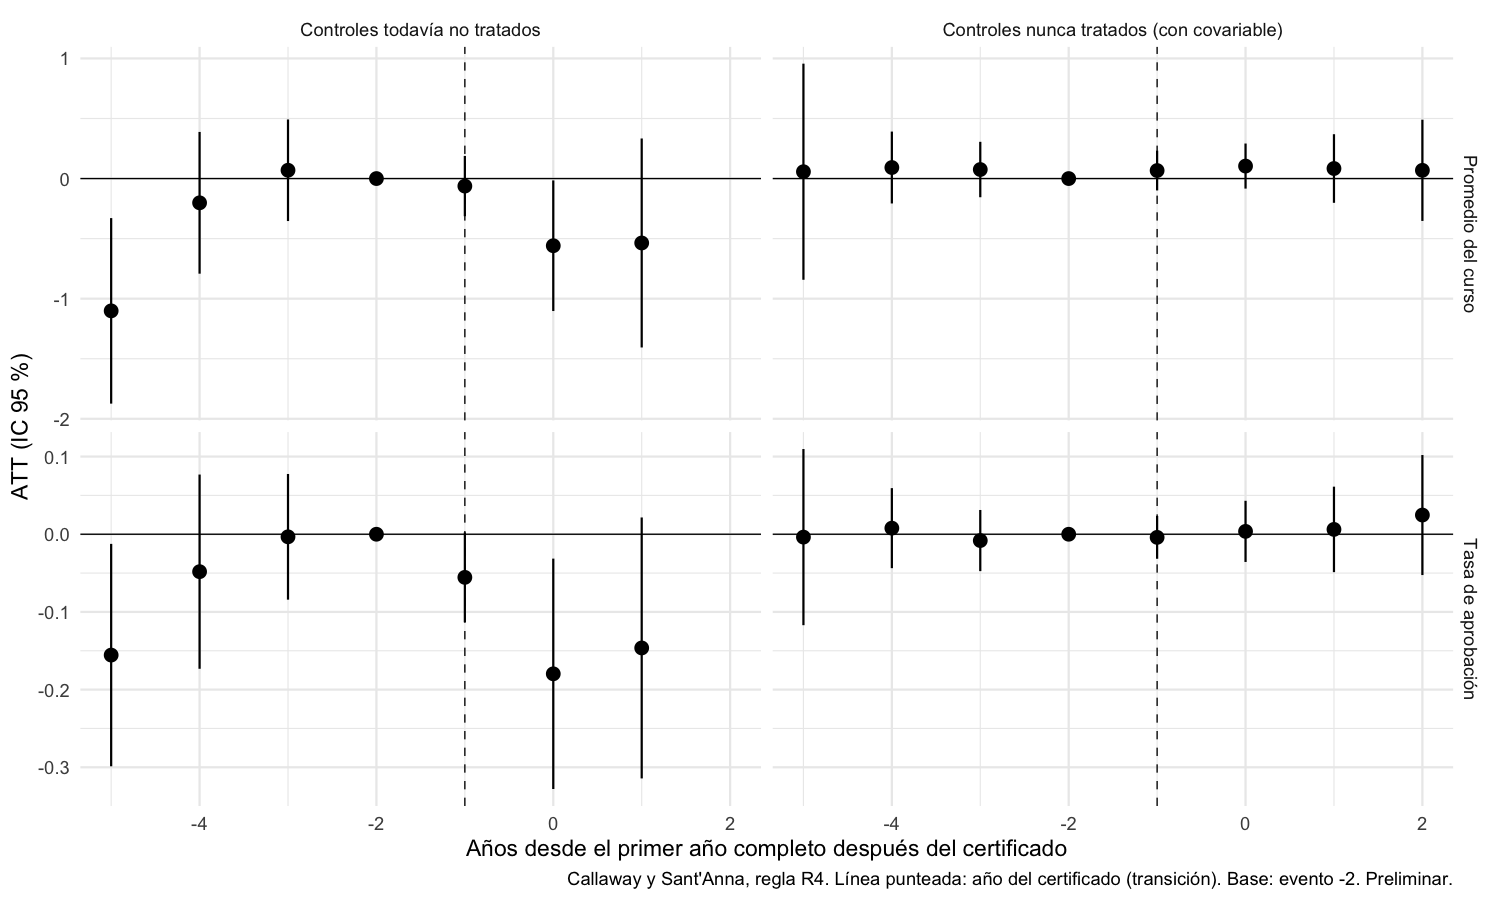
\includegraphics[width=\textwidth]{did_event_study.png}
    \end{column}
    \begin{column}{0.33\textwidth}\scriptsize
      \textbf{Cómo leerlo}
      \begin{itemize}
        \item Cada punto es la diferencia entre docentes del diplomado y controles en ese año, respecto del año $-2$.
        \item Barras: intervalo de 95 \%. Si cruza el cero, no hay diferencia distinguible.
        \item Línea punteada: año del certificado (transición). A su izquierda, los años \textbf{antes} del diplomado, y a su derecha, los años \textbf{después}.
      \end{itemize}
      \textbf{Qué muestra}
      \begin{itemize}
        \item \textbf{Panel ``todavía no tratados'':} pocos controles e intervalos anchos. El punto $-5$ se calcula contra \textbf{un solo docente}. No es concluyente.
        \item \textbf{Panel ``nunca tratados'':} antes de la línea punteada todo está en cero (los grupos evolucionaban parecido), y después también.
      \end{itemize}
    \end{column}
  \end{columns}
\end{frame}

\begin{frame}{¿Qué tan grande tendría que ser el efecto para poder verlo?}
  \begin{table}\small
    \begin{tabular}{lcccc}
      \toprule
      & \multicolumn{2}{c}{Promedio del curso} & \multicolumn{2}{c}{Tasa de aprobación} \\
      & \multicolumn{2}{c}{(puntos de nota)} & \multicolumn{2}{c}{(puntos porcentuales)} \\
      \cmidrule(lr){2-3}\cmidrule(lr){4-5}
      Significancia & 5 \% & 7 \% & 5 \% & 7 \% \\
      \midrule
      Comparando con docentes todavía no tratados & 0,94 & 0,89 & 20 & 19 \\
      Comparando con docentes nunca tratados & 0,33 & 0,32 & 6,3 & 6,0 \\
      \bottomrule
    \end{tabular}
  \end{table}
  {\scriptsize Efecto mínimo detectable con 80 \% de potencia: 2,80 veces el error estándar al 5 \% de significancia y 2,65 veces al 7 \%.}
  \vspace{0.5em}
  \begin{itemize}
    \item Con los controles todavía no tratados, solo detectaríamos efectos enormes, de casi un punto de nota. Es poco realista para una formación docente.
    \item Con los nunca tratados detectaríamos efectos más moderados, pero a cambio de suponer que esos docentes son comparables.
    \item Con estos datos \textbf{no encontramos evidencia de un efecto}, pero eso no prueba que no lo haya: con la comparación más limpia, la muestra todavía no alcanza.
  \end{itemize}
  \sintesis{La pregunta que sí podemos responder hoy}{Hoy la pregunta no es ``¿funciona el diplomado?'', sino ``¿cuántos datos más necesitamos para saberlo?''. Los docentes que empiezan la versión 6 ayudan a responder eso.}
\end{frame}

\begin{frame}{Qué podemos y qué no podemos concluir hoy}
  \begin{columns}[T]
    \begin{column}{0.48\textwidth}
      \begin{block}{Podemos afirmar}
        \begin{itemize}\small
          \item Las bases se pueden conectar con muy poca pérdida (97,8 \%).
          \item Hay 32 docentes del diplomado comparables antes y después.
          \item La tendencia de las notas está muy influida por la expansión de los programas trimestrales.
          \item El procedimiento funciona de punta a punta y se puede volver a correr.
        \end{itemize}
      \end{block}
    \end{column}
    \begin{column}{0.48\textwidth}
      \begin{alertblock}{Todavía no podemos afirmar}
        \begin{itemize}\small
          \item Si el diplomado mejora o no los resultados de los cursos.
          \item Si un cambio en las notas refleja aprendizaje o un cambio en la forma de evaluar.
          \item Cuál es la fecha exacta en que empieza el efecto de cada versión.
        \end{itemize}
      \end{alertblock}
    \end{column}
  \end{columns}
  \vspace{0.5em}
  {\small Los resultados numéricos completos están en la lámina de respaldo. Son \textbf{preliminares} y no deben circular como estimación del efecto.}
\end{frame}

% ============================================================
\section{Validación con el equipo}
% ============================================================

\begin{frame}{Preguntas para ustedes}
  \small
  \begin{enumerate}
    \item \textbf{Encuadre.} ¿El promedio y la tasa de aprobación de los cursos son una aproximación útil a lo que les importa, como primera pieza de un estudio mixto?
    \item \textbf{Secciones con varios docentes.} ¿Les parece razonable atribuir el resultado de la sección a todos sus docentes? ¿Quién pone la nota final?
    \item \textbf{Fechas.} ¿En qué meses empezó y terminó cada versión? ¿La versión certificada en 2023 terminó en qué mes?
    \item \textbf{Versión 6.} ¿Pueden enviarnos a los docentes que inician en noviembre, con el RUT anonimizado igual que en las otras bases? Serían el grupo de comparación más limpio.
    \item \textbf{Tipo de docente.} ¿Incluimos a ayudantes (AY), guías de campo clínico (GC) y actores (SC), o solo a docentes de aula?
    \item \textbf{Significancia.} ¿En su área se trabaja habitualmente con 5 \% o con 7 \%? Cambia poco el efecto mínimo detectable (lámina 18), pero queremos usar su convención.
    \item \textbf{Segundo contexto.} ¿Qué formación usamos para la prueba de sensibilidad? Proponemos una estable y con muchos aprobados, por ejemplo el taller de Gamificación (unos 125 registros) o el de Aprendizaje Basado en Proyectos (unos 116).
  \end{enumerate}
\end{frame}

\begin{frame}{Próximos pasos (entrega el 27 de noviembre)}
  \begin{enumerate}
    \item Incorporar sus respuestas de hoy: la regla para secciones compartidas, el tipo de docente y la formación del segundo contexto.
    \item Cargar las fechas y cohortes de cada versión y los docentes de la versión 6 apenas lleguen. El código ya está preparado para recibirlos.
    \item Replicar el diseño de Angrist y Lavy: comparar cada cohorte del diplomado con docentes que nunca lo hicieron, pero que antes del diplomado eran parecidos (tipo de programa, contrato, escuela principal donde dictan y nivel de notas).
    \item Completar la prueba de trade-off (varios modelos sobre el diplomado) y la de sensibilidad (otra formación).
    \item Entregar el informe y el código documentado para que la unidad pueda volver a correrlo.
  \end{enumerate}
  \vspace{0.6em}
  \begin{block}{Lo que más nos ayudaría}
    Las fechas de cada versión y la lista de docentes de la versión 6 son las dos piezas que más mejoran el análisis.
  \end{block}
\end{frame}

\begin{frame}
  \begin{center}
    {\Large ¡Gracias!}\\[1em]
    Comentarios, dudas y correcciones son muy bienvenidos.
  \end{center}
\end{frame}

% ============================================================
\appendix
\section*{Respaldo}
% ============================================================

\begin{frame}{Respaldo: resultados preliminares completos}
  \begin{table}\scriptsize
    \begin{tabular}{llccccc}
      \toprule
      Especificación & Control & \multicolumn{2}{c}{Promedio del curso} & \multicolumn{2}{c}{Tasa de aprobación} \\
      \cmidrule(lr){3-4}\cmidrule(lr){5-6}
      & & Efecto & Error est. & Efecto & Error est. \\
      \midrule
      Principal: todos los docentes, con peso & Todavía no tratados & $-$0,55 & 0,34 & $-$0,17 & 0,07 \\
      Solo secciones con un docente & Todavía no tratados & $-$0,80 & 0,44 & $-$0,24 & 0,11 \\
      Docente con mayor responsabilidad & Todavía no tratados & $-$0,66 & 0,41 & $-$0,21 & 0,11 \\
      Con covariable de composición & Nunca tratados & 0,09 & 0,12 & 0,008 & 0,022 \\
      Ídem, sin el año previo al certificado & Nunca tratados & $-$0,03 & 0,18 & 0,010 & 0,027 \\
      Sun y Abraham (contraste) & Todavía no tratados & $-$0,12 & 0,10 & $-$0,11 & 0,03 \\
      \bottomrule
    \end{tabular}
  \end{table}
  \vspace{0.3em}
  \begin{itemize}\small
    \item Método: Callaway y Sant'Anna (2021), panel anual docente $\times$ año, año del certificado como transición.
    \item Las estimaciones con controles todavía no tratados se basan en 3 combinaciones cohorte--año y en 6 controles en 2025.
    \item \alert{Preliminar: no usar como estimación del efecto del diplomado.}
  \end{itemize}
\end{frame}

\begin{frame}{Referencias}
  \small
  \begin{itemize}
    \item Angrist, J. D. y Lavy, V. (2001). Does teacher training affect pupil learning? Evidence from matched comparisons in Jerusalem public schools. \emph{Journal of Labor Economics}, 19(2), 343--369.
    \item Callaway, B. y Sant'Anna, P. H. C. (2021). Difference-in-differences with multiple time periods. \emph{Journal of Econometrics}, 225(2), 200--230.
    \item Goodman-Bacon, A. (2021). Difference-in-differences with variation in treatment timing. \emph{Journal of Econometrics}, 225(2), 254--277.
    \item Sun, L. y Abraham, S. (2021). Estimating dynamic treatment effects in event studies with heterogeneous treatment effects. \emph{Journal of Econometrics}, 225(2), 175--199.
  \end{itemize}
\end{frame}

\end{document}
